\documentclass[aspectratio=169,10pt]{beamer}

\usetheme{Madrid}
\usecolortheme{seahorse}

\usepackage[utf8]{inputenc}
\usepackage{amsmath}
\usepackage{amssymb}
\usepackage{amsfonts}
\usepackage{mathtools}
\usepackage{listings}
\usepackage{xcolor}
\usepackage{tikz}
\usepackage{pgfplots}
\pgfplotsset{compat=1.18}

\graphicspath{{figures/}}

% Code listing style
\lstdefinestyle{mypython}{
    language=Python,
    basicstyle=\ttfamily\scriptsize,
    commentstyle=\color{green!50!black}\itshape,
    keywordstyle=\color{blue}\bfseries,
    stringstyle=\color{red},
    numbers=left,
    numberstyle=\tiny\color{gray},
    breaklines=true,
    frame=single,
    rulecolor=\color{black!30},
    columns=fullflexible,
}

% Theorem styles
\setbeamertemplate{theorems}[numbered]
\setbeamertemplate{footline}[frame number]

% Define remark environment
\newtheorem{remark}[theorem]{Remark}

% Colors
\definecolor{myblue}{RGB}{31,119,180}
\definecolor{myorange}{RGB}{255,127,14}
\definecolor{mygreen}{RGB}{44,160,44}
\definecolor{myred}{RGB}{214,39,40}

\title[Ch 2a: Fixed Point Concepts]{Chapter 2a: Fixed Point Concepts}
\subtitle{Differential Calculus in Banach Spaces}
\author{Based on Hemant Kumar Pathak: \\ Introduction to Nonlinear Analysis and Fixed Point Theory}
\date{\today}

\begin{document}

\frame{\titlepage}

% ============================================================================
% Overview Frame
% ============================================================================

\begin{frame}[allowframebreaks]{Overview}
  \tableofcontents
\end{frame}

% ============================================================================
% Section 1: Introduction
% ============================================================================

\section{Introduction to Differential Calculus in Banach Spaces}

\begin{frame}{Why Differential Calculus in Banach Spaces?}
  \begin{itemize}
    \item Classical calculus works in finite-dimensional spaces $\mathbb{R}^n$
    \item Fixed point theory often involves infinite-dimensional spaces
    \item Examples:
      \begin{itemize}
        \item Function spaces: $C[0,1]$, $L^2([0,1])$
        \item Sobolev spaces: $W^{1,2}(\Omega)$
        \item Sequence spaces: $\ell^p$
      \end{itemize}

    \item \textbf{Challenge:} How to extend derivatives to infinite dimensions?

    \item \textbf{Solution:} Two concepts of differentiability
      \begin{enumerate}
        \item Gâteaux derivative (directional)
        \item Fréchet derivative (full differentiability)
      \end{enumerate}
  \end{itemize}

  \vspace{0.5cm}
  \begin{center}
    \textbf{These are essential for fixed point existence theorems!}
  \end{center}
\end{frame}

\begin{frame}{Banach Space Setup}
  \begin{definition}[Banach Space]
    A complete normed linear space $(X, \|\cdot\|)$ where:
    \begin{itemize}
      \item $X$ is a vector space over $\mathbb{R}$ or $\mathbb{C}$
      \item $\|\cdot\|: X \to \mathbb{R}_{\geq 0}$ is a norm
      \item All Cauchy sequences converge (completeness)
    \end{itemize}
  \end{definition}

  \begin{example}
    \begin{itemize}
      \item $\mathbb{R}^n$ with $\|x\|_2 = \sqrt{\sum_{i=1}^n x_i^2}$
      \item $C[0,1]$ with $\|f\|_\infty = \sup_{t \in [0,1]} |f(t)|$
      \item $\ell^p$ with $\|x\|_p = \left(\sum_{i=1}^\infty |x_i|^p\right)^{1/p}$
    \end{itemize}
  \end{example}

  \begin{definition}[Dual Space]
    The dual space $X^*$ is the space of all continuous linear functionals on $X$.
  \end{definition}
\end{frame}

% ============================================================================
% Section 2: Gâteaux Derivatives
% ============================================================================

\section{Gâteaux Derivatives}

\begin{frame}{Definition: Gâteaux Derivative}
  \begin{definition}
    Let $F: X \to Y$ be an operator between Banach spaces. $F$ is \textbf{Gâteaux differentiable} at $x \in X$ if there exists a continuous linear operator $A: X \to Y$ such that:

    \[
      \lim_{t \to 0} \frac{1}{t}\left\|F(x + th) - F(x) - tAh\right\| = 0 \quad \forall h \in X
    \]

    The operator $A$ is called the \textbf{Gâteaux derivative} at $x$, denoted $dF(x)$ or $F'(x)$.
  \end{definition}

  \vspace{0.3cm}
  \textbf{Key interpretation:} Limit is taken \textbf{along each direction} $h$ separately.

  \begin{remark}
    \begin{itemize}
      \item The Gâteaux derivative, if it exists, is \textbf{unique}
      \item It need \textbf{NOT} imply continuity of $F$
      \item It's a directional derivative generalization
    \end{itemize}
  \end{remark}
\end{frame}

\begin{frame}{Example: Discontinuous Gâteaux Derivative}
  \begin{example}[Example 3.1]
    Let $F: \mathbb{R}^2 \to \mathbb{R}$ be:
    \[
      F(x) = \begin{cases}
        \frac{x_1^3}{x_2}, & \text{if } x = (x_1, x_2) \neq (0,0) \\
        0, & \text{if } x = (0,0)
      \end{cases}
    \]

    Then:
    \begin{itemize}
      \item $dF(0) = 0$ (null operator) exists as Gâteaux derivative
      \item But $F$ is \textbf{discontinuous} at $(0,0)$
      \item For any $h = (h_1, h_2) \in \mathbb{R}^2$:
        \[
          dF(0)h = \lim_{t \to 0} \frac{F(th) - F(0)}{t} = \lim_{t \to 0} \frac{2t^3 h_1^3}{t h_2} = 0
        \]
    \end{itemize}
  \end{example}
\end{frame}

\begin{frame}{Gradient and Partial Derivatives}
  \begin{definition}[Gradient]
    For a functional $f: X \to \mathbb{R}$ (real-valued), the mapping $x \mapsto f'(x)$ is called the \textbf{gradient} of $f$ and denoted $\nabla f$. Thus $\nabla f$ is a mapping from $X$ to $X^*$.
  \end{definition}

  \begin{observation}
    For operators $F: \mathbb{R}^n \to \mathbb{R}^m$ with $F = (f_1, f_2, \ldots, f_m)$ and matrix $A = (a_{ij})$:

    The Gâteaux derivative $F'(x)$ has matrix representation (Jacobian matrix):
    \[
      F'(x) = \begin{bmatrix}
        \partial_1 f_1(x) & \cdots & \partial_n f_1(x) \\
        \vdots & \ddots & \vdots \\
        \partial_1 f_m(x) & \cdots & \partial_n f_m(x)
      \end{bmatrix}
    \]
  \end{observation}
\end{frame}

\begin{frame}{Constant and Linear Operators}
  \begin{lemma}
    \begin{enumerate}
      \item The constant mapping $F: X \to Y$ with $F(x) = a$ has Gâteaux derivative $F'(x) = 0$ (the null operator).

      \item Any continuous linear operator $A: X \to Y$ has Gâteaux derivative $A'(x) = A$ for all $x \in X$.
    \end{enumerate}
  \end{lemma}

  \textbf{Proof idea for (2):}

  For linear $A$:
  \[
    \frac{1}{t}\|A(x + th) - A(x) - tAh\| = \frac{1}{t}\|Ax + tAh - Ax - tAh\| = 0
  \]
\end{frame}

% ============================================================================
% Section 3: Fréchet Derivatives
% ============================================================================

\section{Fréchet Derivatives}

\begin{frame}{Definition: Fréchet Derivative}
  \begin{definition}
    An operator $F: X \to Y$ is \textbf{Fréchet differentiable} at $x \in X$ if there exists a continuous linear operator $A: X \to Y$ such that:

    \[
      \lim_{\|h\| \to 0} \frac{\left\|F(x + h) - F(x) - Ah\right\|}{\|h\|} = 0
    \]

    The operator $A$ is the \textbf{Fréchet derivative} at $x$, denoted $dF(x)$ or $F'(x)$.
  \end{definition}

  \vspace{0.3cm}
  \textbf{Key difference from Gâteaux:} The limit is taken in a \textbf{full neighborhood}, not just along directions.

  \begin{remark}
    \begin{itemize}
      \item Fréchet differentiability $\Rightarrow$ Gâteaux differentiability
      \item Fréchet differentiability $\Rightarrow$ Continuity
      \item Converse implications do NOT hold in general
    \end{itemize}
  \end{remark}
\end{frame}

\begin{frame}{Comparison: Gâteaux vs Fréchet}
  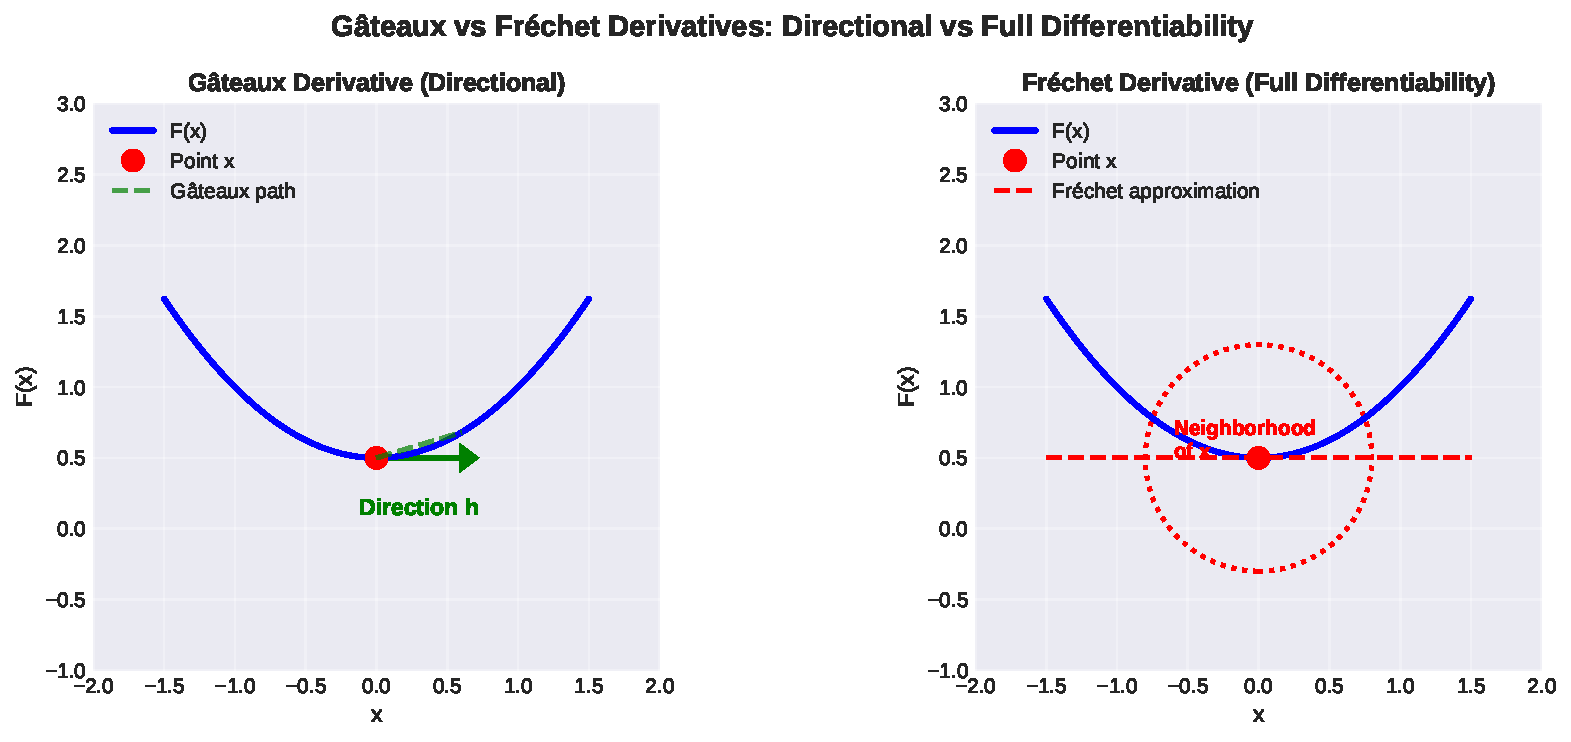
\includegraphics[width=0.95\textwidth]{fig_derivatives_intuition}

  \begin{center}
    {\small Gâteaux: directional limits $\Leftrightarrow$ Fréchet: uniform limit in neighborhood}
  \end{center}
\end{frame}

\begin{frame}[fragile]{Example: Fréchet Continuous but Not Gâteaux Continuous}
  \begin{example}[Example 3.2]
    Let $F: \mathbb{R}^2 \to \mathbb{R}$ be:
    \[
      F(x_1, x_2) = \begin{cases}
        \frac{2x_2 \exp(-x_1^2)}{x_2^2 + \exp(-2x_1^2)}, & x_1 \neq 0 \\
        0, & x_1 = 0
      \end{cases}
    \]

    Then:
    \begin{itemize}
      \item $F$ is Gâteaux differentiable at $(0, 0)$ with $dF(0) = 0$
      \item BUT $F$ is \textbf{NOT continuous} at the origin
      \item Reason: along the path $x = (t, t^2)$, $F(t, t^2) \to 2/e \neq 0$ as $t \to 0$
    \end{itemize}
  \end{example}
\end{frame}

\begin{frame}{Strong Hemicontinuity}
  \begin{definition}
    An operator $F: X \to Y$ is \textbf{strongly hemicontinuous} at $x$ if for every sequence $x_n \to x$ along a line (i.e., $x_n = x + t_n h$ with $t_n \to 0$), we have $F(x_n) \to Fx$.
  \end{definition}

  \begin{theorem}[Theorem 3.5]
    If $F: X \to Y$ is Gâteaux differentiable at $x \in X$, then $F$ is strongly hemicontinuous at $x$.
  \end{theorem}

  \textbf{Proof sketch:}
  \begin{itemize}
    \item If $\phi(t) = F(x + th)$ is differentiable at 0 with $\phi'(0) = F'(x)h$
    \item Then $\phi$ is continuous at 0
    \item So $F(x + t_n h) \to F(x)$ when $t_n \to 0$
  \end{itemize}
\end{frame}

% ============================================================================
% Section 4: Mean Value Theorem
% ============================================================================

\section{Mean Value Theorem for Gâteaux Derivatives}

\begin{frame}{Mean Value Theorem}
  \begin{theorem}[Theorem 3.1 - Mean Value Theorem]
    Let $f: X \to \mathbb{R}$ be a functional with Gâteaux derivative $df(x, h)$ at every point $x \in X$. Then for points $x, x+h \in X$, there exists a constant $\tau \in (0, 1)$ such that:
    \[
      f(x + h) - f(x) = df(x + \tau h, h)
    \]
  \end{theorem}

  \textbf{Key insight:} Extends the classical mean value theorem to Banach spaces!

  \begin{remark}
    In $\dim X > 1$, we generally have \textbf{inequality}, not equality:
    \[
      f(x + h) - f(x) \neq df(x + \tau h, h)
    \]
    for arbitrary compositions of directions.
  \end{remark}
\end{frame}

\begin{frame}{Illustration of Mean Value Theorem}
  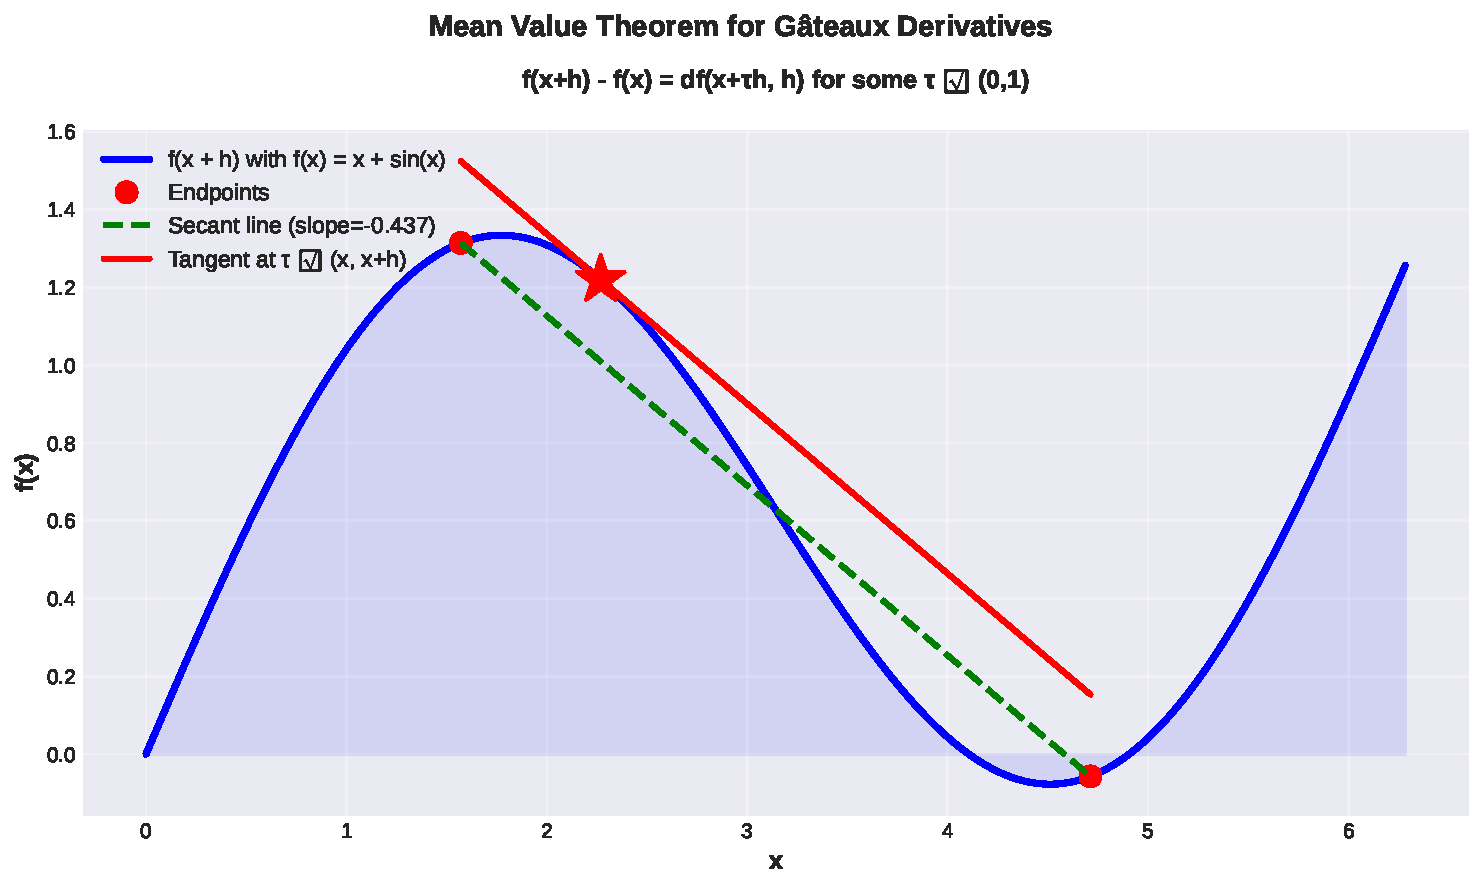
\includegraphics[width=0.95\textwidth]{fig_mean_value_theorem}

  \begin{center}
    {\small For f(x) = x + sin(x): secant and tangent slopes coincide somewhere in between}
  \end{center}
\end{frame}

% ============================================================================
% Section 5: Chain Rule
% ============================================================================

\section{Chain Rule for Derivatives}

\begin{frame}{Chain Rule for Gâteaux and Fréchet Derivatives}
  \begin{theorem}[Theorem 3.6 - Chain Rule]
    Let $X, Y, Z$ be real Banach spaces, $G: X \to Y$ Gâteaux differentiable at $x$, and $F: Y \to Z$ Fréchet differentiable at $G(x)$. Then $H = F \circ G$ is Gâteaux differentiable at $x$ with:
    \[
      H'(x) = F'(G(x)) \circ G'(x)
    \]

    If $G(x)$ is also Fréchet differentiable, then $H'(x)$ is the Fréchet derivative.
  \end{theorem}

  \begin{remark}
    The composition of derivatives:
    \begin{itemize}
      \item $G'(x): X \to Y$ (Gâteaux)
      \item $F'(G(x)): Y \to Z$ (Fréchet)
      \item Product: $F'(G(x)) \circ G'(x): X \to Z$
    \end{itemize}
  \end{remark}
\end{frame}

\begin{frame}{Chain Rule Composition Diagram}
  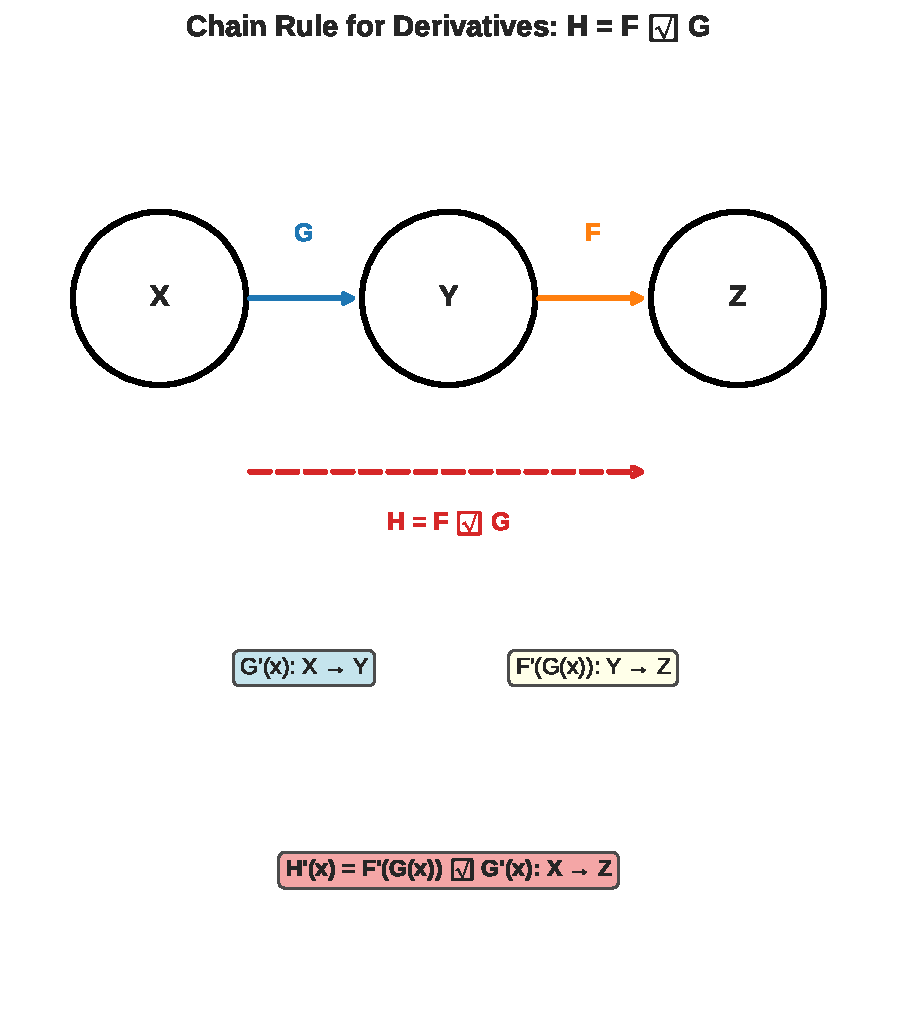
\includegraphics[width=0.95\textwidth]{fig_chain_rule}

  \begin{center}
    {\small Composition of operators and their derivatives follow the chain rule}
  \end{center}
\end{frame}

\begin{frame}{Proof Strategy for Chain Rule}
  For $t \neq 0$:
  \[
    \begin{split}
      &\frac{1}{|t|}\|H(x + th) - Hx - tF'(Gx)G'(x)h\| \\
      &\leq \frac{1}{|t|}\|F(G(x+th)) - F(G(x)) - F'(Gx)(G(x+th) - G(x))\| \\
      &\quad + |F'(Gx)(G(x+th) - Gx - tG'(x)h)|
    \end{split}
  \]

  \begin{itemize}
    \item First term $\to 0$ by Fréchet differentiability of $F$ at $G(x)$
    \item Second term involves continuity of $F'(Gx)$ and Gâteaux diff. of $G$
  \end{itemize}
\end{frame}

% ============================================================================
% Section 6: Subdifferentials
% ============================================================================

\section{Subdifferentials and Convexity}

\begin{frame}{Convexity in Banach Spaces}
  \begin{definition}[Strictly Convex Space]
    A Banach space $X$ is \textbf{strictly convex} if its unit ball $B_X = \{x \in X: \|x\| \leq 1\}$ contains no line segments in its boundary.

    Equivalently: if $\|x\| = \|y\| = 1$ with $x \neq y$, then $\left\|\frac{x+y}{2}\right\| < 1$.
  \end{definition}

  \begin{example}
    \begin{itemize}
      \item $L^2$ norm on $\mathbb{R}^n$: \textbf{strictly convex}
      \item $L^1$ and $L^\infty$ norms: \textbf{NOT strictly convex}
      \item $C[0,1]$ space: \textbf{NOT strictly convex}
    \end{itemize}
  \end{example}
\end{frame}

\begin{frame}{Unit Balls in Different Spaces}
  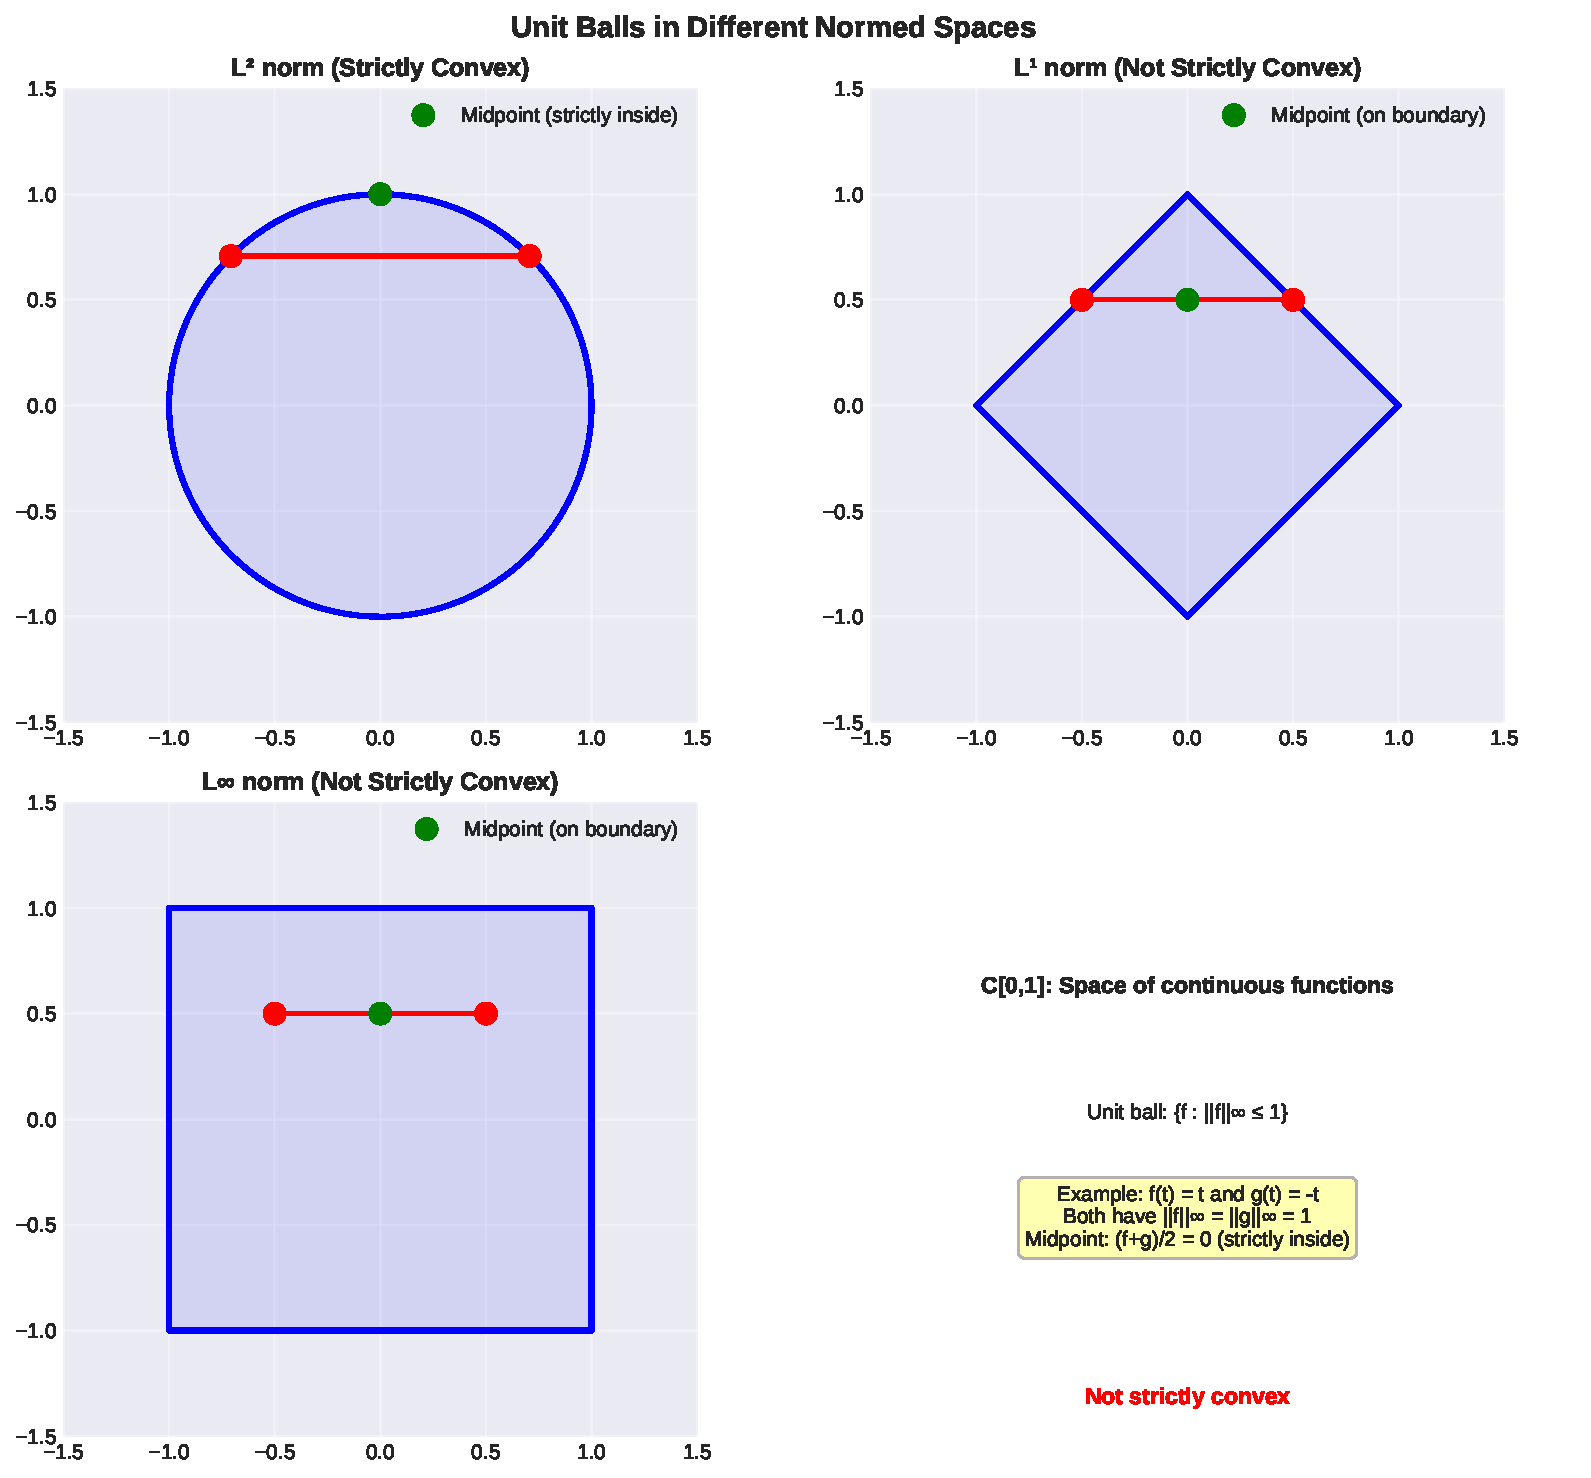
\includegraphics[width=0.95\textwidth]{fig_unit_balls}

  \begin{center}
    {\small Different spaces have different geometric properties}
  \end{center}
\end{frame}

\begin{frame}{Subdifferential Definition}
  \begin{definition}
    For a functional $f: X \to \mathbb{R}$, the \textbf{subdifferential} $\partial f(x)$ at $x \in X$ is the set of all functionals $x^* \in X^*$ such that:
    \[
      f(y) \geq f(x) + \langle x^*, y - x \rangle \quad \forall y \in X
    \]

    Each $x^* \in \partial f(x)$ is called a \textbf{subgradient} at $x$.
  \end{definition}

  \begin{remark}
    \begin{itemize}
      \item For smooth functions: $\partial f(x) = \{\nabla f(x)\}$ (singleton)
      \item For non-smooth convex functions: $\partial f(x)$ is non-empty, closed, convex
      \item Generalizes the gradient to non-differentiable convex functions
    \end{itemize}
  \end{remark}
\end{frame}

\begin{frame}{Subdifferential Illustration}
  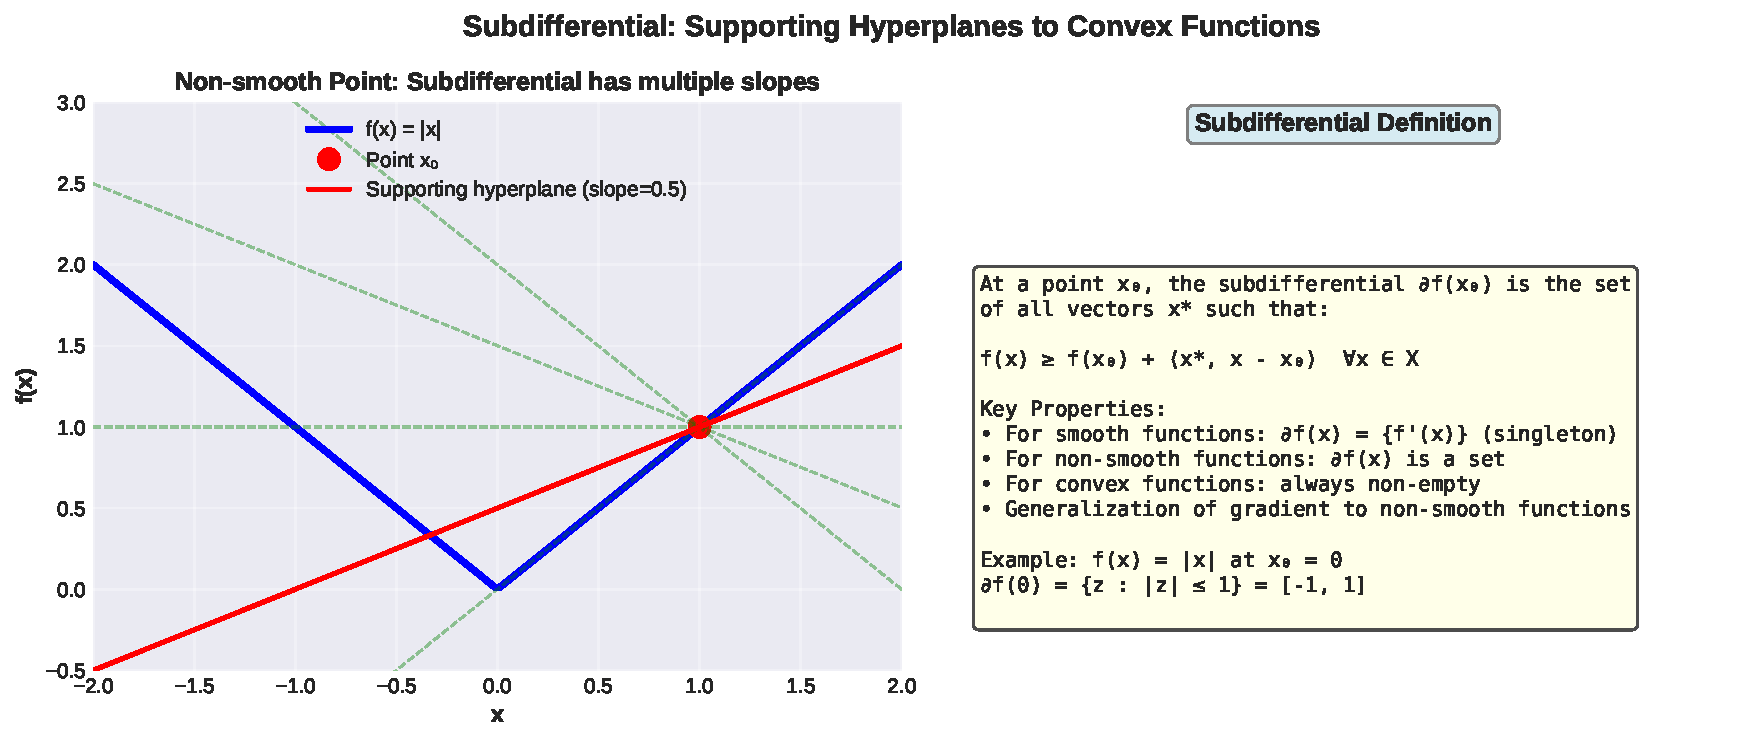
\includegraphics[width=0.95\textwidth]{fig_subdifferential}

  \begin{center}
    {\small Supporting hyperplanes to convex functions: slopes in subdifferential}
  \end{center}
\end{frame}

\begin{frame}[fragile]{Example: Subdifferential of Absolute Value}
  \begin{example}[Norm Functional]
    For the norm functional $f(x) = \|x\|$ on a Banach space $X$:
    \begin{itemize}
      \item At $x \neq 0$: $\partial f(x) = \{x^* \in X^*: \|x^*\|_{X^*} \leq 1, \langle x^*, x \rangle = \|x\|^2\}$

      \item At $x = 0$: $\partial f(0) = B_{X^*} = \{x^* \in X^*: \|x^*\|_{X^*} \leq 1\}$ (closed ball in dual)
    \end{itemize}
  \end{example}

  \begin{example}[Duality Mapping]
    The \textbf{duality mapping} $J: X \to X^*$ is defined as:
    \[
      J(x) = \{x^* \in X^*: \langle x^*, x \rangle = \|x\|^2, \|x^*\| = \|x\|\}
    \]

    For strictly convex spaces, $J$ is single-valued (a function).
  \end{example}
\end{frame}

\begin{frame}{Conjugate Function and Subdifferentiability}
  \begin{definition}
    For $f: X \to \mathbb{R}$, the \textbf{conjugate function} $f^*: X^* \to \mathbb{R}$ is:
    \[
      f^*(x^*) = \sup_{x \in X} \left(\langle x^*, x \rangle - f(x)\right)
    \]
  \end{definition}

  \begin{theorem}[Theorem 3.21 - Fenchel Duality]
    $x^* \in \partial f(x)$ and $x \in \partial f^*(x^*)$ if and only if:
    \[
      \langle x^*, x \rangle = f(x) + f^*(x^*)
    \]
  \end{theorem}

  \textbf{Key consequence:} Subdifferentials are closely linked to duality through conjugate functions.
\end{frame}

\begin{frame}{Subdifferentiability of Convex Functions}
  \begin{theorem}[Theorem 3.22 - Subdifferentiability]
    Let $f$ be a lower semicontinuous function on a Banach space $X$. Then:
    \[
      \mathcal{D}(\partial f) = \mathcal{D}(f)
    \]
    where $\mathcal{D}(\cdot)$ denotes the effective domain (where function is finite).
  \end{theorem}

  \begin{remark}
    For convex functions:
    \begin{itemize}
      \item Subdifferentiable everywhere on interior of domain
      \item May not be differentiable (even Gâteaux)
      \item Subdifferential can be non-empty even at boundary points
    \end{itemize}
  \end{remark}
\end{frame}

\begin{frame}{Subdifferential of Norm Functional}
  \begin{theorem}[Theorem 3.23]
    The subdifferential of the norm functional $j(x) = \frac{\|x\|^2}{2}$ on a Banach space $X$ is precisely the duality mapping $J$:
    \[
      \partial j = J
    \]
  \end{theorem}

  \textbf{Implications:}
  \begin{itemize}
    \item The norm is subdifferentiable everywhere
    \item At non-zero points, subdifferential is unique (for strictly convex spaces)
    \item At zero, subdifferential is the closed ball in the dual space
  \end{itemize}
\end{frame}

% ============================================================================
% Section 7: Applications
% ============================================================================

\section{Applications and Examples}

\begin{frame}{Hammerstein Operator}
  \begin{definition}
    The \textbf{Hammerstein operator} $F: L_p[0,1] \to L_p[0,1]$ is defined as:
    \[
      [Fx](s) = \int_0^1 k(s,t) f(t, x(t)) dt
    \]
    where:
    \begin{itemize}
      \item $k(s,t)$ is a kernel function
      \item $f(t, \cdot)$ is nonlinear in the second argument
    \end{itemize}
  \end{definition}

  \begin{example}[Gâteaux Differentiability]
    Under suitable conditions on $k$ and $f$:
    \[
      dF(x)h = \int_0^1 k(s,t) \frac{\partial f}{\partial u}(t, x(t)) h(t) dt
    \]
    The Gâteaux derivative is the integral operator with kernel and partial derivative.
  \end{example}
\end{frame}

\begin{frame}{Hammerstein Operator Visualization}
  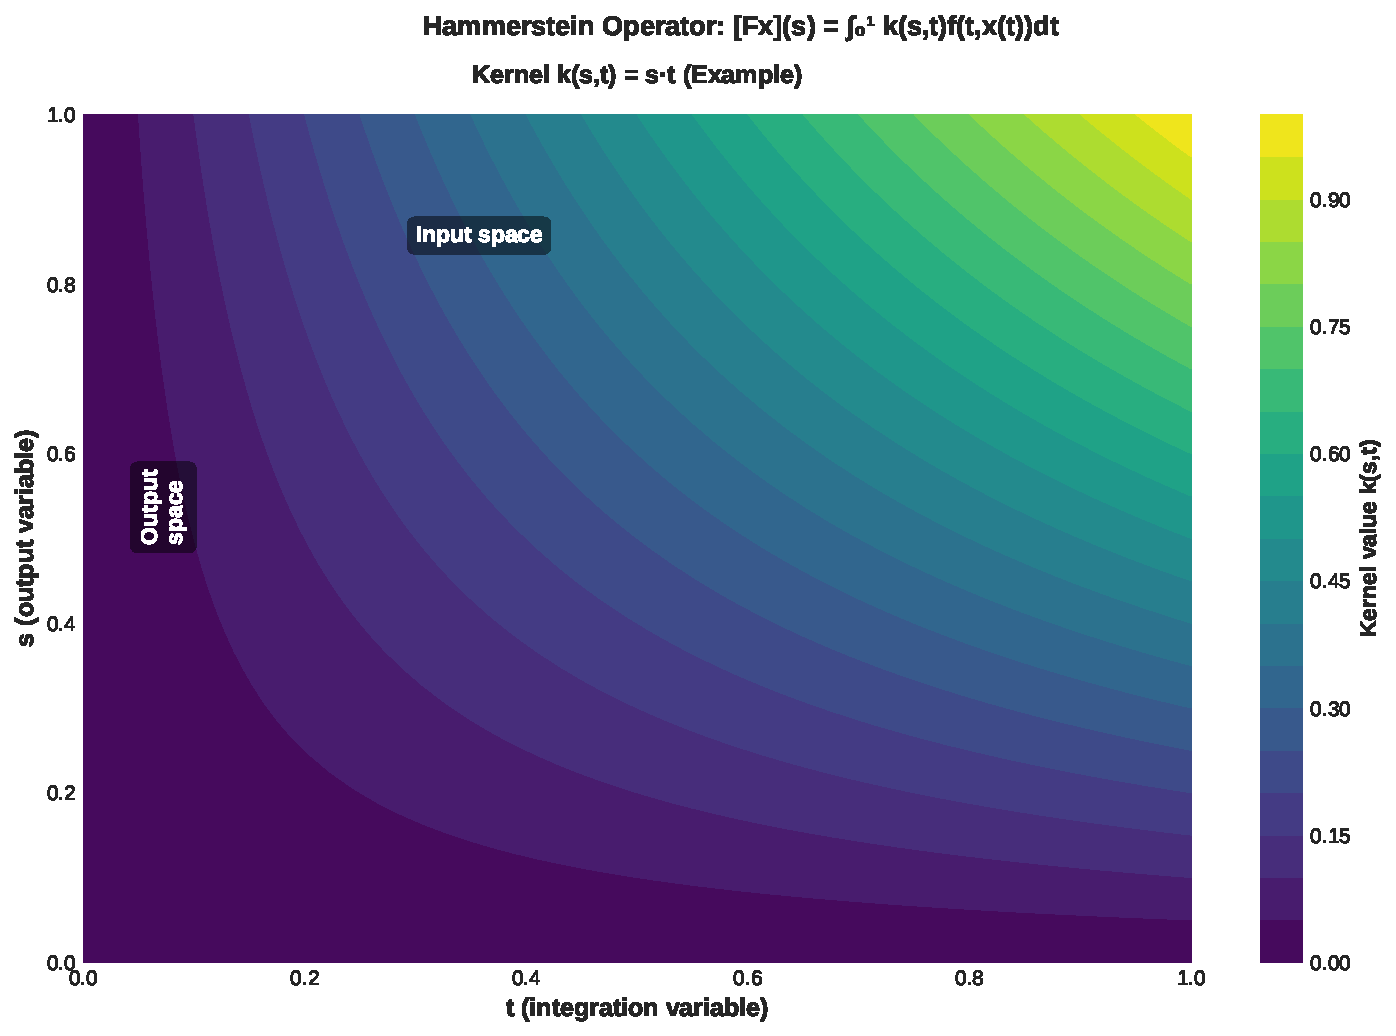
\includegraphics[width=0.95\textwidth]{fig_hammerstein_operator}

  \begin{center}
    {\small Kernel structure: integration variable $t$ and output variable $s$}
  \end{center}
\end{frame}

\begin{frame}[fragile]{Implicit Function Theorem Application}
  \begin{problem}
    Suppose $F: X \times Y \to Z$ is continuously Fréchet differentiable with $F(x_0, y_0) = 0$. If $D_y F(x_0, y_0)$ is invertible, then:
    \begin{itemize}
      \item There exist neighborhoods $U \subset X$, $V \subset Y$
      \item And a unique continuous function $\varphi: U \to V$ with $\varphi(x_0) = y_0$
      \item Such that $F(x, \varphi(x)) = 0$ for all $x \in U$
    \end{itemize}
  \end{problem}

  \textbf{Fixed point perspective:}
  \begin{itemize}
    \item Can be used to prove existence of solutions to equations
    \item Foundation for continuation methods in fixed point theory
    \item Links differential calculus to implicit function existence
  \end{itemize}
\end{frame}

\begin{frame}{Example: Hilbert Space Norm Functional}
  \begin{example}[Example 3.21]
    Let $X$ be a real Hilbert space and $f(x) = \|x\|$ for $x \in X$.
    \begin{itemize}
      \item For $x \neq 0$:
        \[
          \nabla f(x) = \frac{x}{\|x\|}
        \]
        \textbf{Gâteaux differentiable} with this gradient.

      \item At $x = 0$:
        \begin{itemize}
          \item NOT differentiable (singular point)
          \item \textbf{Subdifferentiable}: $\partial f(0) = \{x^* \in X^*: \|x^*\| \leq 1\}$
          \item This is the closed unit ball in the dual
        \end{itemize}
    \end{itemize}
  \end{example}
\end{frame}

\begin{frame}{Indicator Function and Normal Cones}
  \begin{example}[Example 3.23 - Indicator Function]
    For a convex subset $C$ of a Hilbert space $X$:
    \[
      I_C(x) = \begin{cases}
        0, & \text{if } x \in C \\
        \infty, & \text{if } x \notin C
      \end{cases}
    \]

    At boundary point $x_0 \in \partial C$:
    \[
      \partial I_C(x_0) = \{x^* \in X: \langle x^*, x - x_0 \rangle \leq 0 \text{ for all } x \in C\}
    \]
    This is the \textbf{normal cone} to $C$ at $x_0$.
  \end{example}
\end{frame}

% ============================================================================
% Section 8: Concept Hierarchy
% ============================================================================

\section{Summary and Concept Hierarchy}

\begin{frame}{Differential Calculus Concept Hierarchy}
  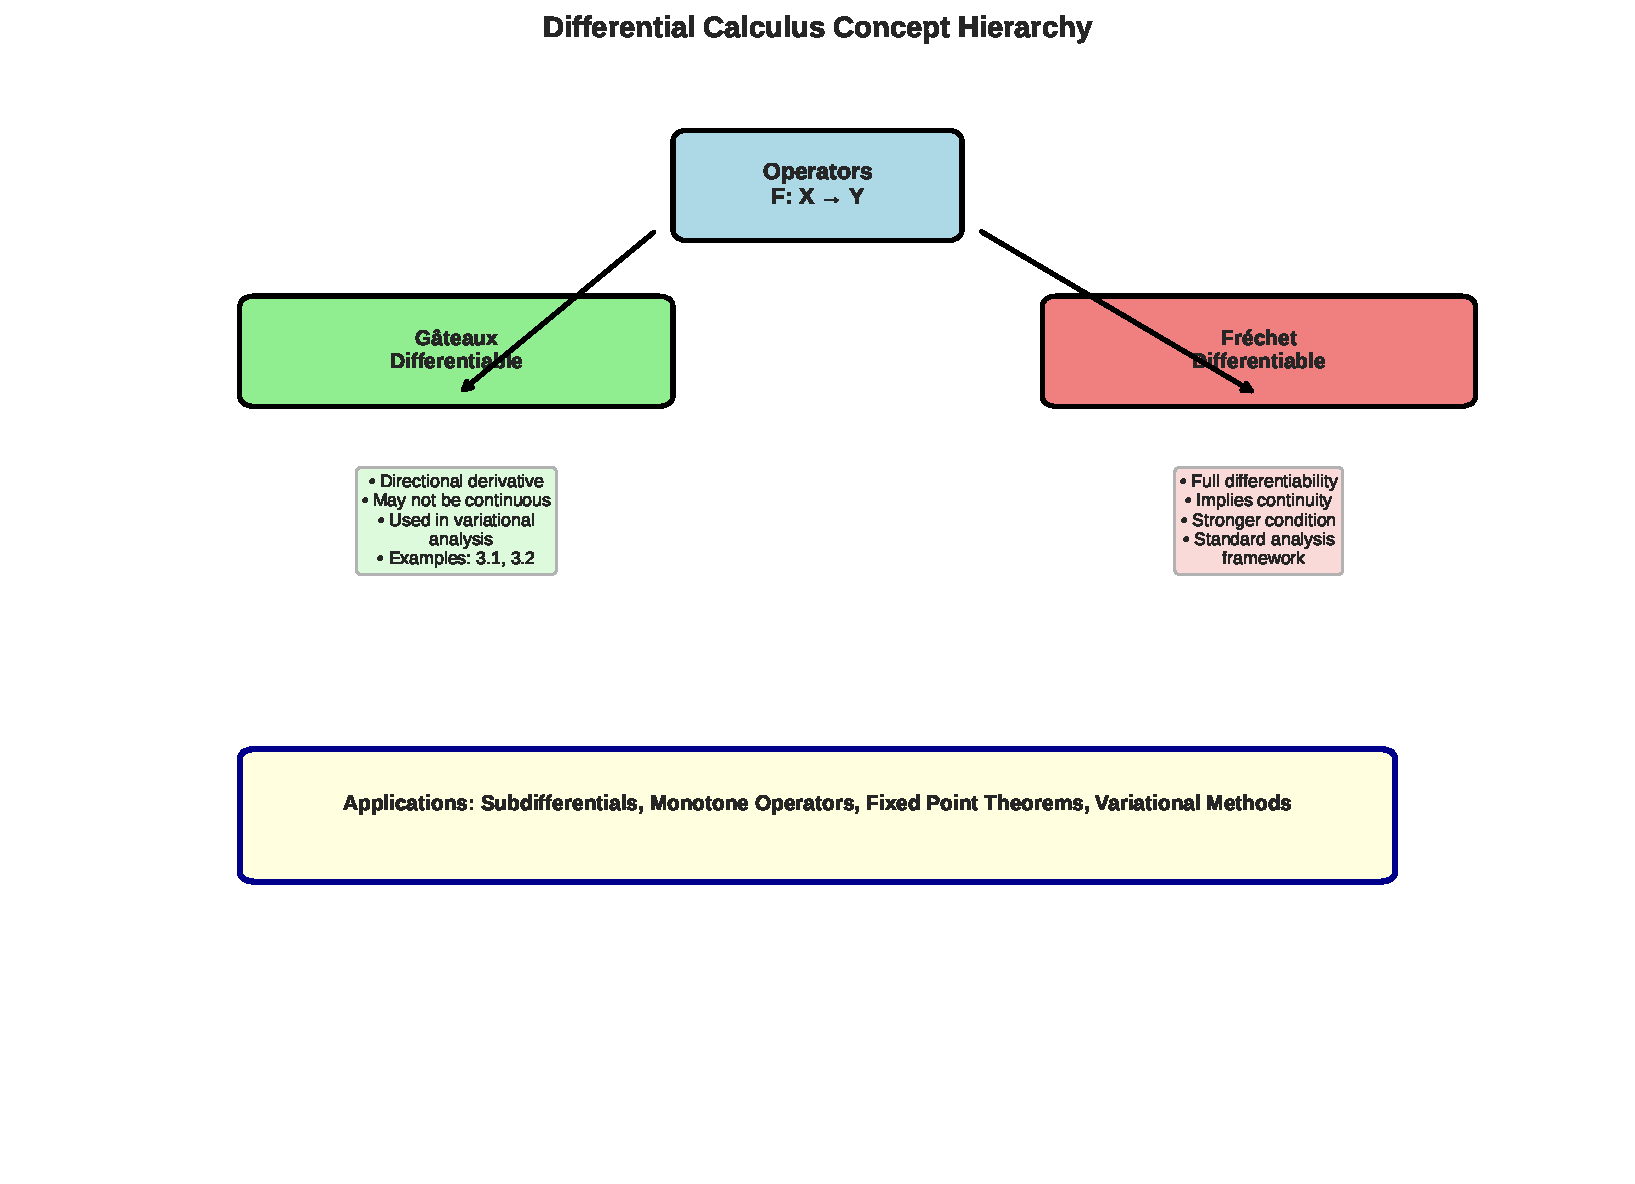
\includegraphics[width=0.95\textwidth]{fig_concept_hierarchy}
\end{frame}

\begin{frame}{Key Definitions Summary}
  \begin{center}
    \begin{tabular}{|l|c|c|}
      \hline
      \textbf{Concept} & \textbf{Banach Space} & \textbf{Related To} \\
      \hline
      Gâteaux Derivative & Directional & Variational Methods \\
      Fréchet Derivative & Full Differentiability & Standard Analysis \\
      Strong Hemicontinuity & Intermediate & Fixed Point Theorems \\
      Subdifferential & Non-smooth Functions & Monotone Operators \\
      Duality Mapping & Dual Space Structure & Banach Space Geometry \\
      \hline
    \end{tabular}
  \end{center}
\end{frame}

\begin{frame}{Connection to Fixed Point Theory}
  \textbf{Why this matters for fixed points:}

  \begin{enumerate}
    \item \textbf{Gâteaux derivatives:} Used in variational formulations
      \begin{itemize}
        \item Fixed point equations as variational problems
        \item Energy functionals and minimization
      \end{itemize}

    \item \textbf{Subdifferentials:} Handle non-smooth fixed point maps
      \begin{itemize}
        \item Proximal operators in iterative methods
        \item Monotone inclusion problems
      \end{itemize}

    \item \textbf{Monotone operators:} Defined via subdifferentials
      \begin{itemize}
        \item $F$ is monotone if $\langle F(x) - F(y), x - y \rangle \geq 0$
        \item Essential for fixed point theorems
      \end{itemize}
  \end{enumerate}
\end{frame}

\begin{frame}{Numerical Example: Computing Derivatives}
  \begin{problem}
    Consider the operator $F: \mathbb{R}^2 \to \mathbb{R}$ with $F(x,y) = x^2 + xy + y^2$.

    Compute the Gâteaux derivative at $(1, 1)$ in direction $h = (1, 0)$.
  \end{problem}

  \textbf{Solution:}
  \[
    \begin{split}
      dF(1,1)(1,0) &= \lim_{t \to 0} \frac{F(1+t, 1) - F(1,1)}{t} \\
      &= \lim_{t \to 0} \frac{(1+t)^2 + (1+t) + 1 - 3}{t} \\
      &= \lim_{t \to 0} \frac{1 + 2t + t^2 + 1 + t + 1 - 3}{t} \\
      &= \lim_{t \to 0} \frac{3t + t^2}{t} = 3
    \end{split}
  \]

  The Jacobian is $\nabla F = (2x + y, x + 2y)$, so $\nabla F(1,1) = (3, 3)$.
\end{frame}

\begin{frame}[allowframebreaks]{References and Further Reading}
  \begin{itemize}
    \item Pathak, H. K. (2018). \textit{Introduction to Nonlinear Analysis and Fixed Point Theory}. Springer.

    \item Zeidler, E. (1986). \textit{Nonlinear Functional Analysis and its Applications}. Springer.

    \item Aubin, J. P., \& Frankowska, H. (1990). \textit{Set-Valued Analysis}. Birkhauser.

    \item Kreyszig, E. (1978). \textit{Introductory Functional Analysis with Applications}. Wiley.

    \item Rockafellar, R. T., \& Wets, R. J. B. (2009). \textit{Variational Analysis}. Springer.
  \end{itemize}

  \vspace{1cm}
  \textbf{Key Topics to Explore Next:}
  \begin{itemize}
    \item Monotone Operators (Chapter 4 in Pathak)
    \item Fixed Point Theorems (Chapter 5 in Pathak)
    \item Topological Degree Theory (Chapter 6 in Pathak)
  \end{itemize}
\end{frame}

\end{document}
